\documentclass[a4paper, 12pt]{article}
%\documentclass{book}

% Important Packages:
 \usepackage{amsmath}    % need for subequations
 \usepackage{amsfonts}
 \usepackage{amsthm}
 \usepackage{graphicx}   % need for figures
 \usepackage{verbatim}   % useful for program listings
 %\usepackage{subfig}  % use for side-by-side figures
 %\usepackage{wrapfig}
 %\usepackage{listings}	 % creates code blocks
 %\usepackage[colorlinks=true]{hyperref}   % use for hypertext links, including
                     % those to external documents and URLs
 %\usepackage{multirow}
 %\usepackage{tikz}
 %\usepackage{enumerate}
 %\usetikzlibrary{decorations.pathreplacing,decorations.pathmorphing}
 %\usetikzlibrary{calc}
 %\usepackage[colorinlistoftodos]{todonotes}
 
 % Useful macros 
 \def\tcb#1{\color{blue}{#1}}
 \def\tcr#1{\color{red}{#1}}	
 \def\tcg#1{\color{green}{#1}}
 \def\be{\begin{eqnarray}}	 	\def\ee{\end{eqnarray}}
 \def\bea{\begin{eqnarray}}	 	\def\eea{\end{eqnarray}}
 \def\bean{\begin{eqnarray*}}	\def\eean{\end{eqnarray*}}
 
 \def\D{\displaystyle}
 \def\T{\textstyle}
 \def\l{\left}
 \def\r{\right}
 \def\nf{n_{\!f}} % quark flavours
 \def\pa{\partial}
 \def\eg{e.\,g.}
 \def\ie{i.\,e.}

 \def\be{\begin{equation}}
 \def\ee{\end{equation}}
 \def\bea{\begin{eqnarray}}
 \def\eea{\end{eqnarray}}
 \def\bean{\begin{eqnarray*}}
 \def\eean{\end{eqnarray*}}
 \def\gsim{\mathrel{\rlap{\lower0.2em\hbox{$\sim$}}\raise0.2em\hbox{$>$}}}
 \def\ksim{\mathrel{\rlap{\lower0.2em\hbox{$\sim$}}\raise0.2em\hbox{$<$}}}
 \def\kg{\mathrel{\rlap{\lower0.25em\hbox{$>$}}\raise0.25em\hbox{$<$}}}
 
 \def\AA{${\buildrel_{\circ} \over {\mathrm{A}}}$}
 \def\bm#1{\mbox{\boldmath$#1$}}
 \newcommand{\eq}[1]{(\ref{#1})} 
 \def\pd{\partial}
 \def\d{\textrm{d}} 
 \def\T{\textstyle}
 \def\eg{e.\,g.}	% exempli gratia (for the sake of example)
 \def\ie{i.\,e.}	% id est (that is)


 % Page configuration:
 \topmargin -2.0cm
 \oddsidemargin -0.85cm
 \evensidemargin -0.85cm
 \textwidth 18cm
 \textheight 24cm
 
\begin{document}
\begin{center}
\textbf{Stellenbosch Camp December 2017 \\ Senior Test 3} \\
\textbf{Solutions}
\end{center}

\begin{enumerate}
    % EGMO 2013 solutions: https://www.egmo.org/egmos/egmo2/solutions.pdf

    % QUESTION 1
    \item[1.] Let
    \[
        n = \prod_{i=1}^{k} p_i^{a_i}
    \]
    be the prime decomposition of $n$. Then the number of divisors of $n$ is
    equal to
    \[
        (a_1 + 1)(a_2 + 1)(a_3 + 1) \cdots (a_k + 1).
    \]

    This must be equal to $9$, and so we can see that $n$ must either be of the
    form $n = p^8$ for some prime number $p$, or of the form $n = p^2 q^2$ for
    some prime numbers $p$ and $q$. It remains to show that both of these cases
    work.

    For $n = p^8$, we have the following arrangement of its factors:
    \[
        \begin{array}{|c|c|c|}
            \hline
            p^3 & p^8 & p \\
            \hline
            p^2 & p^4 & p^6 \\
            \hline
            p^7 & 1 & p^5 \\
            \hline
        \end{array}
    \]

    For $n = p^2 q^2$, we have the following arrangement of its factors:
    \[
        \begin{array}{|c|c|c|}
            \hline
            p^2 q & q^2 & p \\
            \hline
            1 & p q & p^2 q^2 \\
            \hline
            pq^2 & p^2 & q \\
            \hline
        \end{array}
    \]
    
    
    % QUESTION 2
    \item[2.] Let's put segment $MY = MX$ from point $M$ on ray $XM$. Then $\triangle AMY = \triangle MXN$ by an angle and two adjacent edges, now we have:
    \begin{align*}
        P_{ANX} &= AX + XN + AN = AX + AY + MD > XY + MD = 2XM + MD \\
        &> XM + XD + MD = P_{MXD}
    \end{align*}
    as the projection of segment $XD$ into line $AD$ is smaller than the projection of segment $XM$, then the segment itself is smaller by length.
    
    \begin{figure}[h!]
        \centering
        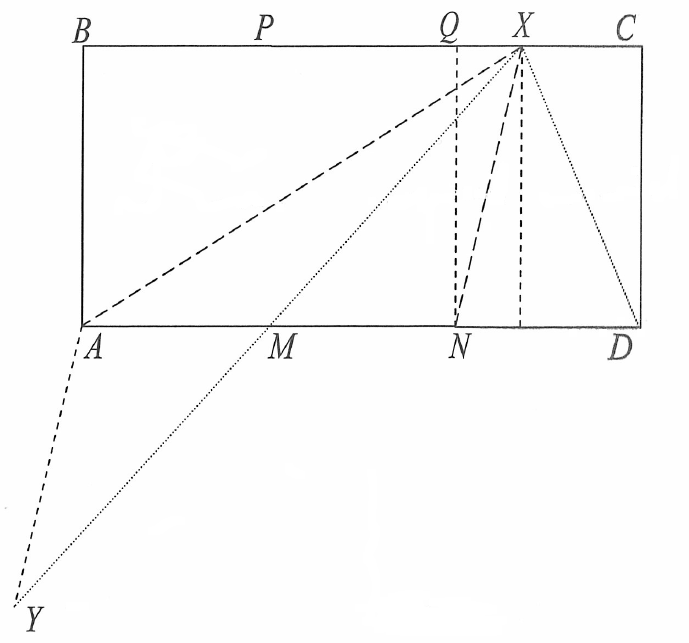
\includegraphics[width=0.4\textwidth]{seniortest3_q3.PNG}
    \end{figure}
    
    
    % QUESTION 3
    \item[3.] Consider the number of pairs of connected lamps with opposite colour, which we call \emph{special pairs}. For each of these pairs, whenever a switch occurs they exchange colours and are still connected and so we see that the number of these special pairs cannot decrease. However, the number of special pairs cannot increase forever, since it is bounded by the total number of pairs, which is finite. Hence after some point onwards the set of pairs of connected lamps with opposite colours stays constant.
    
    From that point onwards, each lamp either forms part of a special pair (in which case it will alternate colours between red and blue, staying the same colour after every two switches) or it does not form part of a special pair and stays that way (in which case its colour stays the same). Either way, from that point onwards each lamp will always have the same colour as it did two switches before that.
    
    
    % QUESTION 4
    \item[4.] Note that if $p=2$ then the given fraction yields 4, which is indeed a perfect square. We now assume $p > 2$. By Bertrand's postulate, there exists a prime $q$, such that $\frac{p-1}{2} < q \leq p-1$. We now consider writing the denominator as a single fraction, where:
    %$$ 1+\frac{1}{2}+\dots+\frac{1}{p-1} = \frac{M}{\textrm{lcm}(1, 2, \dots, p-1)} $$
    \begin{equation} \label{eqn41}
        1+\frac{1}{2}+\dots+\frac{1}{p-1} = \frac{M}{1 \cdot 2 \cdot 3 \cdot \dots (p-1)}
    \end{equation}
    where
    $$ M = \sum_{i=1}^{p-1}  \prod_{k=1, k \neq i}^{p-1} k $$
    Noting that $q$ divides all terms in $M$ except for one, we have that $q \not | M$. Also $q$ divides the denominator of (\ref{eqn41}) exactly once. Hence, the exponent of $q$ in the original fraction is 1, which proves it cannot be a perfect square of a \textit{rational} number if $p>2$.
    
    Hence, only $p=2$ satisfies the desired property.
    

    % QUESTION 5
    \item[5.]  % AoPS, Inequalities Marathon, Problem 25
    \emph{Solution 1:} Note that we have $a^2 + b^2 + \sqrt{c} \geq 2ab + \sqrt{c} = \frac{2}{c} + \sqrt{c}$. Hence, we have
    $$ \sum_\textrm{cyc} \frac {ab}{a^2 + b^2 + \sqrt {c}} \leq \sum_\textrm{cyc} \frac{\frac{1}{c}}{\frac{2}{c} + \sqrt{c}} = \sum_\textrm{cyc} \frac{1}{2 + c\sqrt{c}} $$
    Reducing to a common denominator, we have that:
    \begin{align}
        \sum_\textrm{cyc} \frac{1}{2 + c\sqrt{c}} &= \frac{(2 + b \sqrt{b})(2 + c \sqrt{c}) + (2 + c \sqrt{c})(2 + a \sqrt{a}) + (2 + a \sqrt{a})(2 + b \sqrt{b})}{(2 + a \sqrt{a})(2 + b \sqrt{b})(2 + c \sqrt{c})} \nonumber \\
        &= \frac{4 \cdot 3 + (ab\sqrt{ab} + bc\sqrt{bc} + ca\sqrt{ca}) + 4(a\sqrt{a} + b\sqrt{b} + c\sqrt{c})}{1 + 2(ab\sqrt{ab} + bc\sqrt{bc} + ca\sqrt{ca}) + 4(a\sqrt{a} + b\sqrt{b} + c\sqrt{c}) + 8} \label{eqn51}
    \end{align} 
    
    It now remains to prove that (\ref{eqn51}) $ \leq 1$, where we now use AM-GM:
    $$  ab\sqrt {ab} + bc\sqrt {bc} + ca\sqrt {ca} \geq 3 \sqrt [3]{a^2b^2c^2\sqrt {a^2b^2c^2}} = 3 $$
    which proves that:
    $$ \sum_\textrm{cyc} \frac{1}{2 + c\sqrt{c}} \leq 1 $$
    This completes the proof.
    
	  \emph{Solution 2:} As before, we begin with $a^2 + b^2 + \sqrt{c} \geq 2ab + \sqrt{c} = 2ab + \sqrt{abc^2} = \sqrt{ab}\left(2\sqrt{ab}+c\right)$. Hence, we have
	    \[ \sum_\textrm{cyc} \frac {ab}{a^2 + b^2 + \sqrt {c}} \leq \sum_\textrm{cyc} \frac{\sqrt{ab}}{2\sqrt{ab}+c} = \frac{1}{2} - \frac{c}{4\sqrt{ab}+2c} \]
	  and so it remains to show that
	    \[ \sum_\textrm{cyc} \frac{c}{2\sqrt{ab}+c} \geq 1. \]
	  But by Cauchy's Inequality in Engel form, the left-hand side is
	    \[ \sum_\textrm{cyc} \frac{(\sqrt{c})^2}{2\sqrt{ab}+c} \geq \frac{\left(\sqrt{a}+\sqrt{b}+\sqrt{c}\right)^2}{a+b+c+2\sqrt{ab}+2\sqrt{bc}+2\sqrt{ca}} = 1, \]
	  and so the inequality is proved.
\end{enumerate}
\end{document}





